\chapter{Methodology} \label{method}

\section{Overview of Research Design}

This research adopts a Design Science Research (DSR) methodology to address an operational problem in NHS oncology services: the lack of integrated, actionable visibility of delays between MDT outcomes and treatment initiation. DSR is particuarly suitable for this study because it explicitly focuses on the design, construction, and evaluation of an artefact intended to improve a real-world organisational context, while generating transferable design knowledge \citep{hevner2004}.

The primary artefact developed in this study is a lightweight integrated data repository (IDR) ad decision-support dashboard, designed to consolidate post-MDT pathway data and support operational decision-making. In addition to the artefact itself, the research produces a set of evaluated design principles for oncology operational analytics, constituting a contribution to knowledge beyond the local implementation. 

\subsection{Justification for Design Science Research}
Several methodological approaches were considered. A case study methodology would have enabled detailed examination of post-MDT operational processes but woud not have provided a structured framework for the design and evaluation of an intervention. Action Research was also considered because of its focus on organisational change and practitioner involvement. However, Action Research typically requires repeated cycles of intervention and measurement within live operational environments. In cancer pathway management, allowing breaches to occur in order to evaluate an intervention would be ethically and operationally undesirable given the known relationship between treatment delays and patient outcomes. 

Design Science Research was therfore selected because it provides a rigorous framework for designing, developing, and evaluating an artefact intended to solve a real-world organisational problem while simultaneously generating transferable knowledge. DSR has been widely applied within healthcare informatics, clinical decision support, and data integration research where new technological artefacts are required to address operational challenges \citep{hevner2004, peffers2007}.

Unlike traditional continuous-improvement approaches such as Plan-Do-Check-Act (PDCA), cancer pathway management cannot rely solely on post-hoc measurement of outcomes. A breach of the 31-day or 62-day standard represents a clinically meaningful delay that may adversely affect patient outcomes. Consequently, operational management must emphasise proactive identification and mitigation of risk rather than retrospective evaluation alone. The design objective of the proposed dashboard is therefore not simply to identify breaches after they occur, but to provide leading indicators that enable intervention before delays become clinically significant.

Case study research was rejected because the objective of this study extends beyond understanding operational delays to designing and evaluating a technological intervention intended to address them. Similarly, Action Research was considered unsuitable because it emphasises organisational change through repeated intervention cycles, whereas the primary contribution of this study is the creation and evaluation of an information systems artefact.

\section{Design Science Research Framework}
The study follows the Design Science Research Methodology (DSRM) proposed by \cite{peffers2007}, which structures DSR into six interrelated activities. These activities are applied iteratively rather than strictly linearly. 

\subsection{Problem Identification and Motivation}
The problem identification phase was undertaken using a combination of retrospective pathway analysis, operational observations, and literature synthesis. Local cancer waiting time reports and patient tracking data were reviewed to identify recurring delays between MDT outcomes, first oncology consultation, decision-to-treat, and treatment initiation. Findings were triagulated with evidence from the literature review, which demonstrated similar challenges accross NHS organisations. This process established the need for an integrated operational analytics solution capable of identifying bottlenecks before breaches occur. 

\subsection{Objectives of a Solution}
Solution objectives were derived through a requirements elicitation process combining literature-derived design requirements, operational needs identified through pathway review, and information requirements associated with national cancer waiting time standards. Requirements were grouped into data integration, operational monitoring, decision support, and usability domains.

\subsection{Design and Development}

The design and development stage focused on constructing an Integrated Data Repository (IDR) and a suite of operational decision-support dashboards. Development was undertaken iteratively using successive cycles of prototyping, evaluation and refinement with operational stakeholders. 

The design and development activity involved two tightly coupled components:
\begin{enumerate}
    \item Integrated Data Repository (IDR)
    \item Decision-Support Dashboard
\end{enumerate}
The IDR adopts a general-model architecture consisting of a staging layer for ETL and harmonisation, a central warehouse, and an application layer for analytics and visualisation, consistent with IDR literature for single-institution deployments \citep{gagalova2020}.

The dashboard is designed to support operational tasks rather than retrospective reporting, aligning with the role of operational dashboards in healthcare performance management \citep{buttigieg2017}. 

Both components were developed iteratively, guided by explicit design principles derived from prior research and refined during prototyping. 

\subsubsection{Requirements Elicitation}

Initial requirements were gathered through discussions with operational managers within Portsmouth Oncology Centre, review of existing reporting processes, and analysis of pathway-monitoring activities. Particular attention was paid to identifying operational questions that could not be answered efficiently usng existing systems. 

Key requirements included:
\begin{itemize}
    \item identification of patients at risk of breaching national waiting-time standards;
    \item monitoring active oncology referrals and outstanding clinic activity;
    \item visibility of radiotherapy demand and capacity;
    \item identification of bottlenecks between referral and treatment initiation; and
    \item provision of near-real-time operational decision support.
\end{itemize}

\subsubsection{Source System Analysis}

Four primary operational datasets were identified, and three were used in the final artefact.

The oncology referral register consisted of a manually maintained SharePoint list used by administrative staff to track incoming referrals and clinical outcomes. 

Oncology clinic activity was extracted from the Trust's Patient Administrative System (PAS), providing appointment, booking and attendance data.

Radiotherapy operational data comprised referral, CT simulation and treatment events extracted from the local Oncology Information System - Aria for Radiation Oncology. 

Due to additional projects involving the local Cancer Network, a reliable data source for SACT treatment is not available until January 2027, and was therfore excluded at this time, but design principles leave including SACT treatments at a later date. 

\subsubsection{Data Integration Strategy}

A key design decision concerned the method by which operational data would be extracted from heterogeneous source systems. Alternative approaches including direct database connections, JSON-based exports, application programming interfaces (APIs), and manual reporting extracts were considered. However, functionality varied considerably between source systems. While some systems supported direct database access and others allowed JSON exports, comma-separated value (CSV) export functionality was available consistently across all source applications.

A CSV-based ingestion strategy was therefore adopted to maximise interoperability and minimise source-system dependencies. This approach allowed a common extraction process to be implemented across all datasets while avoiding the need for system-specific integration methods. The resulting architecture prioritised simplicity, portability, and maintainability over real-time integration, which was considered appropriate for an operational dashboard refreshed on a daily basis.

\subsubsection{ETL Architecture and Data Harmonisation}

Data extraction, transformation and loading processes were developed using Python and PostgreSQL. Individual ETL processes were created for each source dataset and orchestrated through an automated pipeline. The ETL layer was responsible for importing source extracts, performing data quality checks, standardising formats, and loading records into the staging layer of the IDR.

The architecture followed a layered design consisting of: 

\begin{itemize}
    \item Source systems;
    \item ETL and harmonisation processes;
    \item Staging tables;
    \item Intermediate integration views;
    \item Analytics-ready fact tables; and
    \item Power BI dashboards.
\end{itemize}

This seperation of concerns simplified troubleshooting, improved transparency, and preserved data lineage throughout the repository. 

The architecture deliberately seperated raw operational data from analytical representations. Staging tables preserved source extracts in their original form, intermediate views applied business rules and data-quality controls, and fact tables provided analytics-ready datasets for dashboard consumption. This separationreduced coupling between source systems and reporting outputs while supporting auditability and future extension of the repository (See Figure \ref{fig:LogicalArch}). 

\begin{figure}
    \centering
    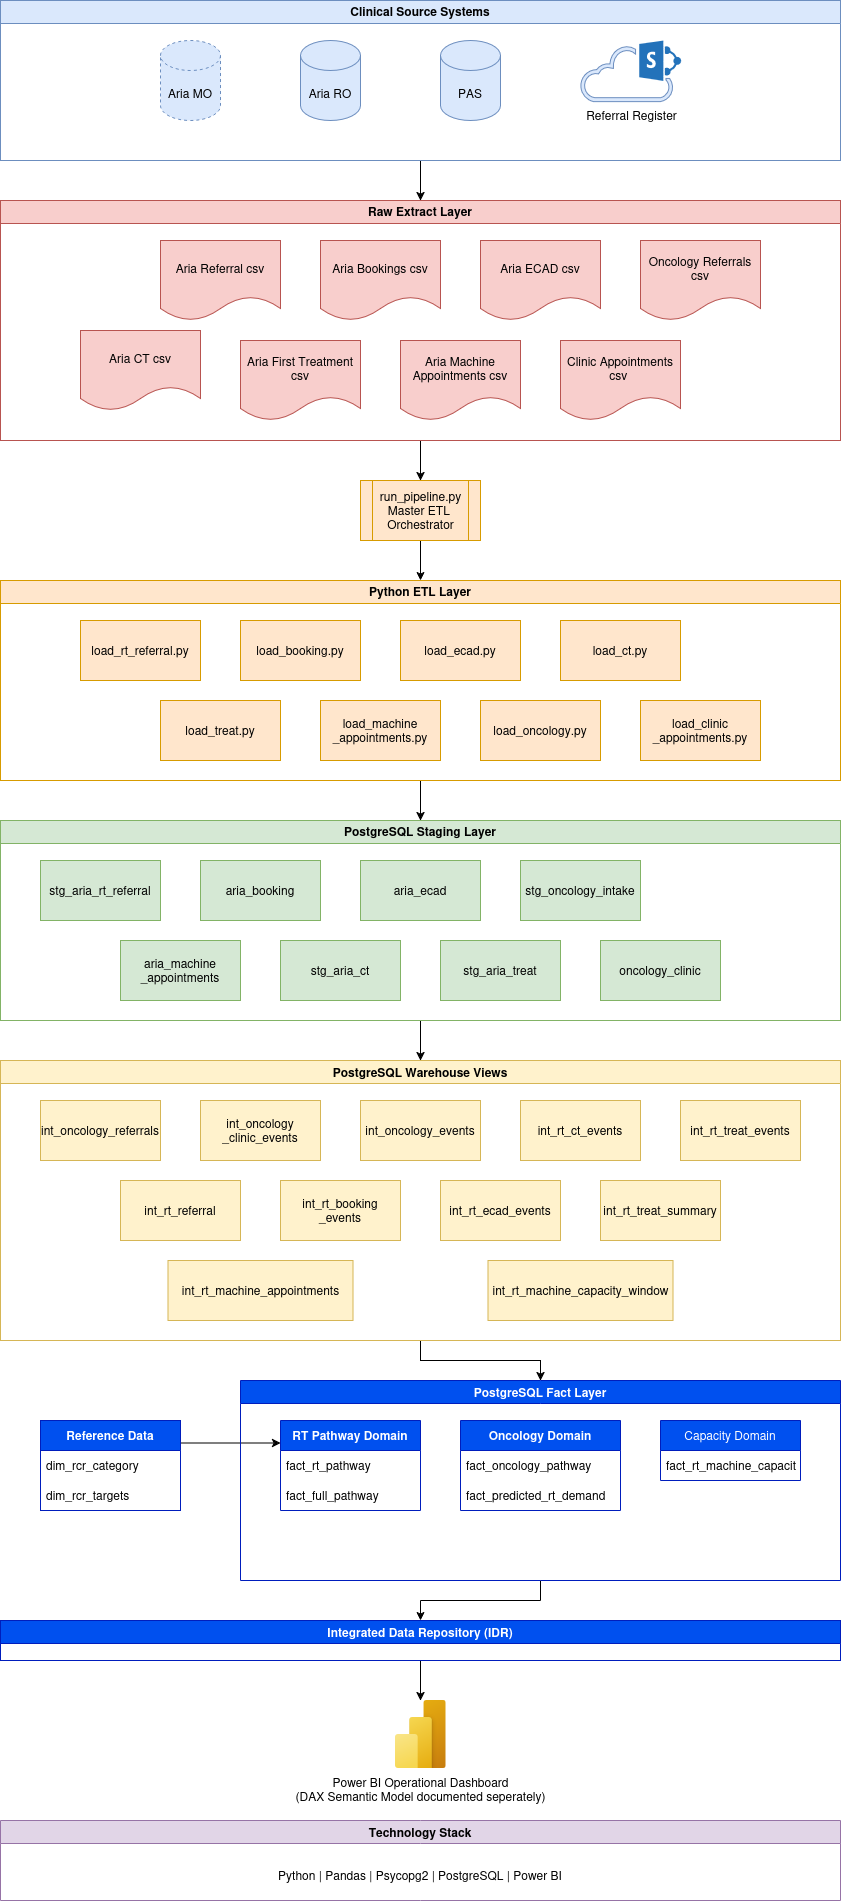
\includegraphics[width=0.5\linewidth]{LogicalArchitecture.png}
    \caption{Logical Architecture of the Integrated Data Repository}
    \label{fig:LogicalArch}
\end{figure}

\subsubsection{Software Engineering and Operational Design}

Although the artefact was developed as a research prototype, several software-engineering practices were incorporated to improve reliability and maintainability.

Logging was implemented throughout the ETL process to support monitoring, troubleshooting, and auditability. All major extractions, transformation and loading activities produced structured log entries allowing operational issues to be investigated retrospectively.

Database credentials and configuration settings were externalised through environment variables rather than being embedded directly within the application code. This approach aligns with principles outlined within the Twelve-Factor App methodology, seperating configuration from code and reducing the risk of credential exposure. 

Togetherm these practices improved operational robustness and facilitated deployment accross development and production environments without modification to application source code. 


\subsection{Pathway Data Model}

\begin{figure}
    \centering
    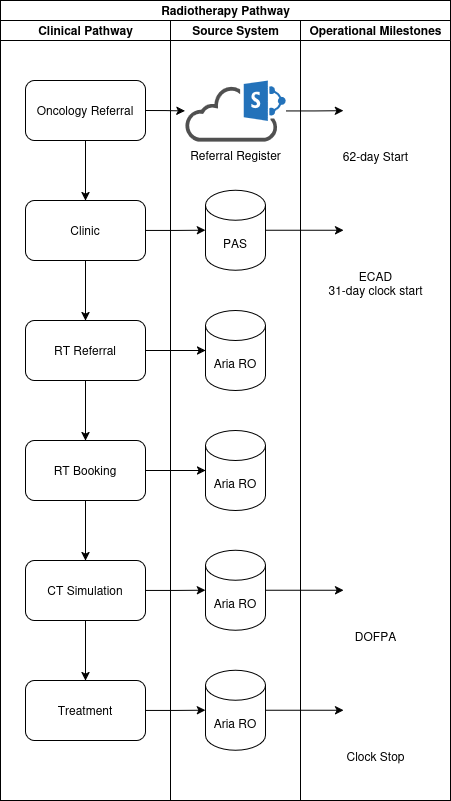
\includegraphics[width=0.5\linewidth]{RTPathwayDataLineage.png}
    \caption{Radiotherapy Pathway, Source Systems and Performance Milestones}
    \label{fig:RTpath}
\end{figure}

The purpose of the pathway data model was to transform fragmented operational records into a series of standardised pathway events capable of supporting interval analysis. A key challenge identified during development was individual source systems recorded only portions of the over all oncology pathway. Consequently, no single source provided a complete end-to-end view from referral to treatment initiation. 

The pathway model therefore adopted a canonical event-based approach. Individual operational events were mapped to a common set of pathway milestones including referral receipt, oncology triage, first clinic appointment, radiotherapy referral, CT simulation, and treatment commencement. These events were subsequently linked through patient identifiers and temporal matching logic to create an integrated representation of each patient pathway. 

From these canonical events, a series of operational intervals were derived, including referral-to-triage, triage-to-clinic, clinic-to-radiotherapy referral, radiotherapy referral-to-CT simulation, and CT simulation-to-treatment. These intervals formed the basis of all dashboard metrics and pathway analyses. 

The use of standardised pathway events aligned with Design Principle 3, ensuring that all metrics were derived consistently across source systems and remained traceable to their originating records. Figure \ref{fig:RTpath} illustrates the relationship between pathway events, source systems, and derived performance milestones.

\subsubsection{Dashboard Development}

Three operational dashboards were developed using Microsoft Power BI. Each dashboard was designed to support a distinct operational management task while sharing a common data repository and data model. 

The Oncology Referrals dashboard focused on referral management activities and provided visibility of active referrals, clinic waiting times, booking lead times, and unresolved clinic outcomes. The dashboard combined referral-register data with clinic activity to provide a current operational view of patients progressing through the oncology pathway. 

The Radiotherapy Service Health dashboard focused on treatment delivery and capacity management. Operational metrics included active patients, expected future referrals, booking backlog, patient risk categorisation, and projected capacity utilisation. Particular emphasis was placed on presenting risk information alongside capacity and demand metrics to support operational intervention. 

The Post-MDT Pathway Overview dashboard integrated data from both oncology and radiotherapy workflows to provide an end-to-end view of patient progression from referral to treatment. The dashboard visualised pathway intervals, operational bottlenecks, and trends in pathway performance over time. 

A fourth dashboard addressing Systemic Anti-Cancer Therapy (SACT) pathways was identified during requirements elicitation. However, due to the lack of a reliable and stable SACT data source during the study period, this component was deferred for future development.

\subsubsection{Iterative Artefact Refinement}
Artefact development followed an iterative process consistent with Design Science Research principles. Successive prototypes were demonstrated to operational stakeholders, with feedback being incorporated into later design iterations. 

The first development cycle focused on radiotherapy operational management. Initial prototypes concentrated on patient tracking and waiting-time performance; however, stakeholder feedback identified a need for greater visibility of future demand and available treatment capacity. This led to the development of capacity-demand forecasting visuals and booking risk indicators. 

The second development cycle focused on oncology referral management. Early versions primarily reported referral volumes and clinic activity. User feedback indicated a stronger operational requirement for active waiting-list management, prompting the addition of patient-group classifications, current booked waits, and referral worklists prioritised by waiting time. 

The third development cycle focused on integrated pathway analysis. Stakeholders identified a need to understand where delays accumulated across the patient journey rather than within individual operational areas. This resulted in the development of pathway-stage metrics and a cumulative waterfall visual illustrating time spent between referral, triage, clinic attendance, radiotherapy referral, CT simulation, and treatment initiation. 

These iterative refinements ensured that the artefact remained closely aligned with operational requirements while simultaneously providing evidence regarding the effectiveness of the proposed design principles.

\subsubsection{ETL and Data Harmonisation}
Data harmonisation presented a significant challenge due to variation in identifier quality, inconsistent recording practices, and differences in operational workflows between source systems. 

NHS numbers were used as the primary identifier wherever possible and were standardised during transformation to remove formatting inconsistencies. Date formats were similarly harmonised to support accurate interval calculations across systems. 

The oncology referral dataset presented particular challenges because it functioned as an operational activity log rather than a controlled referral register. Multiple records were frequently associated with the same oncology episode, reflecting administrative updates, onward referrals, and pathway exceptions. Intermediate transformation views were therefore developed to consolidate records and create a single analytical representation of each referral episode. 

Additional business rules were implemented to identify external-provider referrals, duplicate records, deferred follow-up appointments, and non-standard pathways. These rules allowed operational reporting to focus on patients actively progressing through the pathway while preserving the underlying source data for audit purposes. 

Following transformation and quality-control activities, analytics-ready fact tables were constructed for oncology pathways, radiotherapy pathways, and integrated referral-to-treatment pathways. These fact tables formed the data source for all dashboard visualisations and performance metrics.

\subsection{Data Quality Management}

Exploratory analysis identified several data-quality challenges including duplicate referral records, delayed administrative updates, missing appointment outcomes, and inconsistent coding practices. Rather than modifying source data directly, data-quality controls were implemented within the transformation layer of the repository. 

Business rules were used to identify duplicate referral episodes, exclude non-standard pathways from operational waiting-time calculations, and classify clinician-directed surveillance appointments separately from active patient pathways. This approach preserved the fidelity of source data while improving the validity and interpretability of analytical outputs. 

Data-quality findings were also treated as a research outcome in their own right, providing insight into the operational limitations of existing pathway-monitoring processes and informing recommendations for future pathway digitisation initiatives.

\section{Design Principles} \label{DP}
Design principles represent the design knowledge contribution of this study. They are formulated using a standard DSR structure: \emph{context, intervention}, and \emph{rationale}. These initial principles are refined following evaluation.

\subsection*{DP1: Surface Breach Risks as a Leading Indicator}
If operational teams must prioritise actions in time-constrained cancer pathways, then dashboards should surface leading indicators of breach risk (e.g. days remaining to breach thresholds), because prospective visibility enables earlier and more effective intervention than retrospective compliance metrics. 

\subsection*{DP2: Pair Risk Information with Actionable Capacity Data}
If users are expected to act on identified risks, then risk indicators should be presented alongside relevant capacity and demand information, because risk awareness without visible operational levers does not support decision-making.

\subsection*{DP3: Use Canonical, Standard-Aligned Pathway Events}
If pathway metrics are to be trusted and comparable, then all intervals should be derived from canonical event definitions aligned to NCWTMDS rules, because inconsistent definitions undermine credibility and evaluation validity. 

\subsection*{DP4: Match Data Refresh Cadence to the Action Horizon}
If decisions depend on short operational windows, then data refresh frequency should be aligned to the decision horizon (e.g. daily or near–real-time where feasible), because stale information degrades decision quality.

\subsection*{DP5: Preserve Data Provenance and Auditability}
If analytics are deployed in regulated healthcare environments, then all derived metrics must maintain transparent provenance to source systems, because trust, governance, and reconciliation are essential for adoption.

\subsection*{DP6: Align Interaction Design with Real Operational Tasks}
If dashboards are intended to support complex operational work, then interaction design should reflect users’ real task sequences, because task-aligned interfaces reduce cognitive load and improve decision quality \citep{internationalorganizationforstandardization2020}.

These principles directly inform both the IDR architecture and the dashboard design, and serve as evaluation criteria in Section \ref{EvalStrat}.

\section{Evaluation Strategy} \label{EvalStrat}

Evaluation combines formative and summative methods across four dimensions.

\subsection{Usability Evaluation}
\begin{itemize}
    \item System Usability Scale (SUS)
    \item Heuristic review grounded in ISO 9241-110
    \item Think-aloud walkthroughs
\end{itemize}

\subsection{Utility and Effectiveness}
\begin{itemize}
    \item Task-based experiment with operational users
    \item Primary measures:
    \begin{itemize}
        \item time-to-answer key operational questions,
        \item accuracy of breach-risk identification,
        \item decision quality in constrained scheduling scenarios
    \end{itemize}
\end{itemize}

\subsection{Technical Validity}
\begin{itemize}
    \item Reconciliation of dashboard metrics with source SQL queries
    \item Validation of interval derivations against NCWTMDS rules
\end{itemize}

\subsection{Design Knowledge Evaluation}
\begin{itemize}
    \item Synthesis of user feedback and performance outcomes
    \item Refinement and confirmation of final design principles
\end{itemize}

\section{Ethical and Governance Considerations}
The study operates within UK GDPR and NHS data governance requirements. All data are de-identified or pseudonymised, with access controls and separation between operational and research use. The project follows university ethics procedures and local Trust information governance guidance.

\subsection{Research Limitations}

\begin{itemize}
    \item \textbf{Single-site study:} The artefact will be developed and evaluated within a single NHS Trust, which may limit generalisability.
    \item \textbf{Data quality and availability:} Findings depend on the completeness and accuracy of source systems.
    \item \textbf{Retrospective data:} Restrospective data may not fully represent future operational conditions.
    \item \textbf{Usability sample size:} Evaluation participants are likely to represent a relatively small operational user population. 
    \item \textbf{Artificial evaluation environment:} Demonstration scenarios may not fully replicate live decision-making environments.
    \item \textbf{DSR limitation:} Evaluation assesses utility and usability rather than directly measuring improvements in patient outcomes.
\end{itemize}
\section{Summary}
This chapter has outlined a rigorous, design-science-based methodology that supports both artefact creation and theory-driven knowledge contribution. By embedding explicit design principles within the DSR framework and evaluating the artefact using multiple complementary methods, the study ensures methodological robustness, practical relevance, and academic contribution.
